\documentclass[aspectratio=169]{beamer}

%\includeonly{fig/fig-reper, fig/fig-plav, fig/fig-chung}
%%%%%%%%%%%%%%%%%%%%%%%%%%%%%%%%%%%%%%%%%%%%%%%%%5
%Packages and library
%%%%%%%%%%%%%%%%%%%%%%%%%%%%%%%%%%%%%%%%%%%%%%%%%5

\usepackage[canadien]{babel}
\usepackage[backend=biber, autolang=none, style=authoryear, doi=false, url=false, isbn=false]{biblatex}
\usepackage{pgfplots}
\usepgfplotslibrary{groupplots}
\usetikzlibrary{backgrounds}
\usepackage{vdr}
\usepackage{palettechum}
\usepackage{logovdr}
\usepackage{logochum}
\usetikzlibrary{external}
\tikzsetexternalprefix{pdffig/}
%\tikzexternalize

%%%%%%%%%%%%%%%%%%%%%%%%%%%%%%%%%%%%%%%%%%%%%%%%%5
%Styling
%%%%%%%%%%%%%%%%%%%%%%%%%%%%%%%%%%%%%%%%%%%%%%%%%5

\setbeamertemplate{navigation symbols}{}

\AtBeginSection[]{
	\begin{frame}
		\tableofcontents[currentsection]
	\end{frame}
}

\usefonttheme{structurebold}
\useoutertheme{default}

\setbeamercolor{normal text}{bg=grischum!20}
\setbeamertemplate{itemize item}[square]
\setbeamertemplate{section in toc}[sections numbered]

\setbeamercolor{frametitle}{fg=marinechum, bg=grischum!60}
\setbeamercolor{title}{fg=bleufoncechum}
\setbeamercolor{structure}{fg=marinechum}

%\AtBeginSection[]{
%	\begin{frame}
%		\tableofcontents[currentsection]
%	\end{frame}
%}

\pgfplotsset{
	every axis/.style={
		axis background/.style={fill=white}
	},
	every axis plot/.style={
		mark=none,
	},
	cycle list={
		{bleufoncechum},
		{vertchum},
		{marinechum}
	}
}

\pgfplotsset{
	schoolbook/.style={
		enlargelimits=upper,
		axis lines*=left,
		axis line style={->},
		axis background/.style={
			fill=none
		}
	}
}

\setbeamercovered{transparent=40}


\addbibresource{references.bib}

\title{Le ventilateur VDR-4}
\subtitle{Ventilation convective-diffusive}
\author{Nicolas Blais St-Laurent \tiny{inh}}
\institute{Service d'inhalothérapie}
\date{Automne 2019}
\titlegraphic{\resizebox{!}{1.2cm}{\logochum}\color{structure.fg}\hfill\logofvc{1.2cm}}

\begin{document}


\begin{frame}
\maketitle
\end{frame}

\begin{frame}{Plan de la présentation}
\tableofcontents
\end{frame}

%%%%%%%%%%%%%%%%%%%%%%%%%%%%%%%%%%%%%%%%%%%%%%%%%%%%%%%%%%%%%%%%%%%%%%%%%%%%%
\section{Description du mode de ventilation}
%%%%%%%%%%%%%%%%%%%%%%%%%%%%%%%%%%%%%%%%%%%%%%%%%%%%%%%%%%%%%%%%%%%%%%%%%%%%%

\begin{frame}{Courbe pression-temps typique}
	\centering
		\begin{tikzpicture}
		\begin{axis}[
				width=\textwidth,
				height=0.7\textheight,
				enlarge y limits=upper,
				enlarge x limits=false,
				xmax=8,
				xlabel=Temps (sec.),
				ylabel=Pression (hPa)
				]

			\addplot table [y=Pao ] {dat/simvent1.dat};
		\end{axis}
	\end{tikzpicture}

\end{frame}

\begin{frame}{Haute et basse fréquence}
	\tikzstyle{plage}=[<->, shorten <=0.25mm, shorten >=0.25mm]

\tikzset{
	zoomline/.style={
		opacity=.5,
		dotted
	},
}

\def\zstart{7.2}
\def\zend{7.8}
\def\istart{2}
\def\tic{2}
\def\pstart{7.365}
\def\tip{0.059}

\tikzsetnextfilename{lfhf}
\begin{tikzpicture}
	\begin{groupplot}[
			group style={
				group size=1 by 2,
				y descriptions at=edge left,
				xlabels at=edge bottom
			},
			ylabel=Pression (hPa),
			xlabel=Temps (s),
			max space between ticks=40,
			height= 0.42\textheight,
			enlarge y limits={value=0.9, upper},
			enlarge x limits=false
		]

		\nextgroupplot[
			width=\textwidth]

		\addplot table[x=time, y=Pao] {dat/simvent1.dat};


		\coordinate (PSO) at (axis cs:\zstart,0);
		\coordinate (PSE) at (axis cs:\zend,0);
		\coordinate (PNO) at (axis cs:\zstart,\pgfkeysvalueof{/pgfplots/ymax});
		\coordinate (PNE) at (axis cs:\zend,\pgfkeysvalueof{/pgfplots/ymax});

		\draw [plage](axis cs:\istart,45) -- (axis cs:\istart + \tic, 45) node[midway, above] {Inspi.};
		\draw [plage](axis cs:\istart + \tic,45) -- (axis cs:\istart + 2*\tic, 45) node[midway, above] {Expi.};

		\draw [dashed] 
		(axis cs: \istart,\pgfkeysvalueof{/pgfplots/ymax}) -- (axis cs:\istart,0)
	 	(axis cs: \istart + \tic,\pgfkeysvalueof{/pgfplots/ymax}) -- (axis cs:\istart + \tic,0)
		(axis cs: \istart + 2 *\tic,\pgfkeysvalueof{/pgfplots/ymax}) -- (axis cs:\istart + 2*\tic,0);

		\draw [zoomline] (PSO) rectangle (PNE);


		\nextgroupplot[
				max space between ticks=80,
				width=0.75\textwidth,
				axis background/.style={fill=gray!15, opacity=0.8},
				]

		\addplot +[
			restrict x to domain=\zstart:\zend
			] table[x=time, y=Pao] {dat/simvent1.dat};

		\coordinate (ZNO) at (axis cs:\zstart,\pgfkeysvalueof{/pgfplots/ymax});
		\coordinate (ZNE) at (axis cs:\zend,\pgfkeysvalueof{/pgfplots/ymax});
		\coordinate (ZSO) at (axis cs:\zstart,\pgfkeysvalueof{/pgfplots/ymin});
		\coordinate (ZSE) at (axis cs:\zend,\pgfkeysvalueof{/pgfplots/ymin});


		\draw [dashed] 
		(axis cs: \pstart,\pgfkeysvalueof{/pgfplots/ymax}) -- (axis cs:\pstart,0)
		(axis cs: \pstart + \tip,\pgfkeysvalueof{/pgfplots/ymax}) -- (axis cs:\pstart + \tip,0)
		(axis cs: \pstart + 2 *\tip,\pgfkeysvalueof{/pgfplots/ymax}) -- (axis cs:\pstart + 2*\tip,0);

		\draw [plage] (axis cs:\pstart,45) -- (axis cs:\pstart + \tip, 45) node[midway, above] {Insp.};
		\draw [plage](axis cs:\pstart + \tip,45) -- (axis cs:\pstart + 2*\tip, 45) node[midway, above] {Exp.};

	\end{groupplot}

	\begin{scope}[
			%on background layer
		]
		\fill [opacity=0.075](PSO) rectangle (PNE);
		\draw [zoomline](ZNO) -- (PNO) (PNE) -- (ZNE) ;
		\draw [zoomline](ZSO) -- (PSO) (PSE) -- (ZSE) ;
	\end{scope}

\end{tikzpicture}

\end{frame}

\begin{frame}{Le phasitron}
	\begin{columns}
	\column{0.5\textwidth}
	\begin{block}{Insuflation}
		\vspace{.25cm}
	\begin{tikzpicture}[
			scale=.60,
			every node/.style={transform shape}
			]

	\pic [name=P, draw=black!50, fill=gray!10] {phasitron-coupe};
	\pic {venturi-avance};
	\path (P-S) -- (P-Pt) 
		node [pos=0.32] (J) {}
		coordinate [pos=0.15] (D)
		;


		\draw [structure, line width=.2mm, ->] (P-S) ++(3mm,0) to (D);
		\draw [
			structure, 
			line width=.2mm,
			->, 
shorten <=1mm,
			] (D) to (J);

		\draw [
			structure, 
			line width=.5mm, 
			->, 
			out=90, 
			in=-45,
			shorten >=1mm
		] (P-A) ++ (0, -3mm)  to (J);

		\draw [structure, line width=1mm, ->] (J)  to (P-Pt);
	
\end{tikzpicture}
	\end{block}

%%%%%%%%%%%%%%%%%%%%%%%%%%%%%%%%%%%%%%%%%%%%%%%%%%%%%%%%%5
%%%%%%%%%%%%%%%%%%%%%%%%%%%%%%%%%%%%%%%%%%%%%%%%%%%%%%%%%5

	\column{0.5\textwidth}
	\begin{block}{Expiration}
		\vspace{.25cm}

	\begin{tikzpicture}[
			scale=.60,
			every node/.style={transform shape}
			]

	\pic [name=P, draw=black!50, fill=gray!10] {phasitron-coupe};
	\pic {venturi-recule};

		\draw [
			structure,
			line width=1mm, 
			->, 
			out=0, 
			in=90, 
			looseness=1.8,
			] ([yshift=-4mm]P-Pt) to (P-E);

\end{tikzpicture}
	\end{block}
\end{columns}

\end{frame}

\begin{frame}{Amplification variable}
	\centering
\begin{tikzpicture}
\begin{axis}[
enlargelimits=false,
xlabel=Pression \tiny{($cmH_2O$)},
ylabel=Ratio $\frac{Appel\ d'air}{Air\ inject \acute{e}}$,
ytick={0,1,2,3,4,5},
xtick={0,10,20,30,40},
width=0.4\textwidth,
height={},
title=Ratio d'appel d'air théorique du phasitron,
axis lines=left,
enlargelimits={0.2, upper},
font=\small
]
	\addplot [mark=none] coordinates {(0,5) (40,0)};
\end{axis}
\end{tikzpicture}
\footcite{Percussionairecorporation2009}

\end{frame}

\begin{frame}{Pression alvéolaire}
	\centering
	\begin{tikzpicture}
\begin{axis}[
	width=\textwidth,
	height=0.7\textheight,
	enlarge y limits=upper,
	enlarge x limits=false,
	xmax=8,
	xlabel=Temps (sec.),
	ylabel=Pression (hPa),
	legend=true,
	legend image post style={mark=none}
]

	\addplot table [mark=none, y=Pao ] {dat/simvent1.dat};
\addlegendentry{Pcirc}
	\addplot table [mark=none, y=Palv ] {dat/simvent1.dat};
\addlegendentry{Palv}

\end{axis}
\end{tikzpicture}

\end{frame}

\begin{frame}{Pression motrice}
	\centering
	\newcommand{\pexp}{5}
\newcommand{\pins}{18}
\newcommand{\arrpos}{1.57}
\def\aShift{4.1cm}

\begin{tikzpicture}
	\begin{axis} [
			height=0.80\textheight,
			width=0.75\textwidth,
			extra y ticks={\pexp, \pins},
			extra y tick labels={$P_{exp. moy.}$, $P_{insp. moy.}$},
			xtick={0,2,4},
			ytick={0,30},
			axis x line=bottom,
			axis y line=middle,
			enlarge y limits={0.2, upper},
			extra y tick style={
				grid=major, 
			},
			major grid style={
			}
		]

		\addplot +[
			restrict x to domain=0:4,
			]table[x=time, y=Pao] {dat/simvent1.dat};

		\coordinate (A) at (axis cs:\arrpos,\pexp);
		\coordinate (B) at (axis cs:\arrpos,\pins);
	\end{axis}
		\draw [
			very thick,
			->,
			shorten >=1mm, 
			shorten <=1mm, 
			font=\small
		](A) -- (B) node [pos=0.6, left=3mm, rounded corners, thin]{$P_{motrice}$};

\end{tikzpicture}

\end{frame}

\begin{frame}
	\frametitle{Caractéristiques du mode de ventilation}
	\begin{itemize}
		\item Haute et basse fréquence simultanée
		\item Adaptation dynamique aux changements de mécanique pulmonaire
		\item Respiration spontanée permise
		\item Expiration passive
	\end{itemize}
\end{frame}

%%%%%%%%%%%%%%%%%%%%%%%%%%%%%%%%%%%%%%%%%%%%%%%%%%%%%%%%%%%%%%%%%%%%%%%%%%%%%
\section{Intérêt du mode de ventilation}
%%%%%%%%%%%%%%%%%%%%%%%%%%%%%%%%%%%%%%%%%%%%%%%%%%%%%%%%%%%%%%%%%%%%%%%%%%%%%

\begin{frame}
	\frametitle{Bénéfices escomptés}

	\begin{itemize}
		\item Ventilation protectrice
		\item Désencombrement
		\item Recrutement
	\end{itemize}

\end{frame}

\begin{frame}
	\frametitle{Études randomisées}
	\begin{table}
%	\caption{Études randomisées}
	\begin{tabular}{l l c p{5cm}}

\hline
Auteur	&	Année	&	$n$	& Clientèle\\
\hline
	Chung	&	2010	&	62	&	Grands brûlés, hôpital militaire\\
	Lucangelo	&	2009	&	44	&	Pneumonectomie (intra-op.)\\
	Bougatef	&	2007	(1989)	&	52	&	Prématurés\\
	Reper	&	2002	&	35	&	Brulure d'inhalation\\
	Platteau	&	1999	&	24	&	Chir. card. minimalement inv. (intra-op.)\\
		Hurst	&	1990	&	113	&	SDRA\\
\hline

\end{tabular}
\end{table}

\end{frame}

\begin{frame}
	\frametitle{Séries de cas}
	\begin{table}
%	\caption{Études non randomisées}
	\begin{tabular}{l c c l}

\hline
		Auteur	&	Année	&	$n$	& Clientèle	\\
\hline
		Salim	&	2004	&	10	&	Trauma cranien en SDRA\\
		Oribabor	&	2018	&	24	& P.O. Chir. card.\\
\hline

\end{tabular}
\end{table}

\end{frame}

\begin{frame}
	\frametitle{Chung et al. 2010}

	\begin{block}{Caractéristiques:}

	\begin{itemize}
		\item Étude randomisée
		\item VDR-4 \textit{versus} ventilation protectrice
		\item $n=60$
	\end{itemize}
	\end{block}

	\begin{block}{Résultats:}

	\begin{itemize}
		\item Mortalité et durée de ventilation inchangée
		\item Oxygénation améliorée ($p < .05$)
		\item Pression de crête et moyenne moins élevée
		\item Moins de barotrauma (0 \textit{vs} 4, $p=.04$)
		\item Moins de recours à une thérapie de secours
		\item Étude interrompue sur une analyse interrimaire
	\end{itemize}
	\end{block}

\end{frame}

\begin{frame}{Amélioration de l'oxygénation}
	\centering
		\begin{tikzpicture}
		\begin{axis}[
				height=\textwidth,
				width=1.1\textwidth,
				xlabel=Temps (Jours),
				ylabel=$P_aO_2 / F_iO_2$,
				grid=both,
				ymin=0,
				enlarge x limits=false,
				]
			\addplot table [y=HFPV] {dat/Chung-rounded.csv};
			\addplot table [y=LTV] {dat/Chung-rounded.csv};
			\legend{HFPV, LTV};
		\end{axis}
	\end{tikzpicture}

\end{frame}

\begin{frame}{Amélioration de l'oxygénation}
	\centering
		\begin{tikzpicture}
		\begin{axis} [
				width=\textwidth,
				height=0.7\textheight,
				xlabel=Temps (Jours),
				ylabel=$P_aO_2 / F_iO_2$,
				grid=both,
				ymin=0,
				xmin=0,
				xtick={0,1,...,5},
				enlarge x limits=false,
			%	legend=true,
			%	legend image post style={mark=none}
				]
			\addplot table [y=HFPV, x expr=\thisrow{x}/24] {dat/Reper-rounded.csv};
			\addplot table [y=CMV, x expr=\thisrow{x}/24] {dat/Reper-rounded.csv};
			\legend{HFPV, CMV};
		\end{axis}
	\end{tikzpicture}
	%\footcite{Reper2002}

\end{frame}

%%%%%%%%%%%%%%%%%%%%%%%%%%%%%%%%%%%%%%%%%%%%%%%%%%%%%%%%%%%%%%%%%%%%%%%%%%%%%
\section{Le VDR-4 au CHUM}

\subsection{Considérations pratiques}

\begin{frame}{Le VDR-4 au CHUM}
	\begin{itemize}
		\item Un seul appareil dans l'hôpital
		\item {\em Três} petite équipe d'inhalo formés
		\item Ordonnance collective
		\item Protocole
	\end{itemize}
\end{frame}


\subsection{Protocole clinique}

\begin{frame}
	\frametitle{Paramètres de base}
	\centering
		\begin{tabular}{l r l}
		\hline
		Paramètre & \multicolumn{2}{c}{Valeur}\\
		\hline
		Fperc						&500&/min\\ 
										&(8	&hz)\\
		$P_{exp. moy.}$	&5	&$cmH_2O$\\
		$P_{motrice}$		&10	&$cmH_2O$\\
		$T_{haut}$			& 2	&secondes\\
		$T_{bas}$				& 2	&secondes\\
		\hline
	\end{tabular}

\end{frame}

\begin{frame}
	\frametitle{Gestion de l'oxygénation}
	\centering
		\begin{tikzpicture}
		\begin{axis}[
				height=0.7\textheight,
				xlabel=$F_iO_2$ (\%),
				ylabel=PEP (hPa)
				]

			\addplot +[mark=*] table {dat/oxygenation.dat};
			\node [pin={[align=left]135:$\uparrow T_I$ à 2,4 sec.\\$\downarrow T_E$ à 1.6 sec.}] at (axis cs:100,11){};
		\end{axis}
	\end{tikzpicture}

\end{frame}

\begin{frame}
	\frametitle{Gestion de l'hypercapnie}
	\centering
	\begin{enumerate}
		\item $\downarrow F_{perc}$ \it{ad} 300/min.
		\item $\uparrow T_{inspi.}$ à 3 sec. et $\downarrow T_{expi.}$ à 1 sec.
		\item $\uparrow P_{motrice}$ \it{ad} 20 $cmH_2O$
	\end{enumerate}
\end{frame}

\begin{frame}
\frametitle{Références}
	\printbibliography{}
\end{frame}

\appendix

\section{Fonctionnement de l'appareil}

\begin{frame}{Cartouche pneumatique}
	\begin{columns}
	\column{0.48\textwidth}
	\begin{block}{Cartouche ouverte}
		\vspace{.25cm}
	\begin{tikzpicture}
		\pic [name=C] {cartouche};
		\pic {obturateur-bas};

		\draw [double distance=5.3mm,]
		(CO) -- ++(2,0) (CO) ++ (1,0) |- (CS)
		node [pos=0.25] {$\downarrow$}
		node [pos=0.75] {$\leftarrow$}
		;

		\draw (CI) node {$\downarrow$};
		\draw (CO) node {$\rightarrow$};

	\end{tikzpicture}
	\end{block}

	\column{0.48\textwidth}

	\begin{block}{Cartouche fermée}
		\vspace{.25cm}
	\begin{tikzpicture}

		\pic [name=C] {cartouche};
		\pic {obturateur-haut};

		\draw [double distance=5.3mm,]
		(CO) -- ++(2,0) (CO) ++ (1,0) |- (CS) 
		;

		\draw (CI) node {$\downarrow$};

	\end{tikzpicture}
	\end{block}
\end{columns}

\end{frame}

\begin{frame}[b]
	\frametitle{Circuit logique}
	\centering
	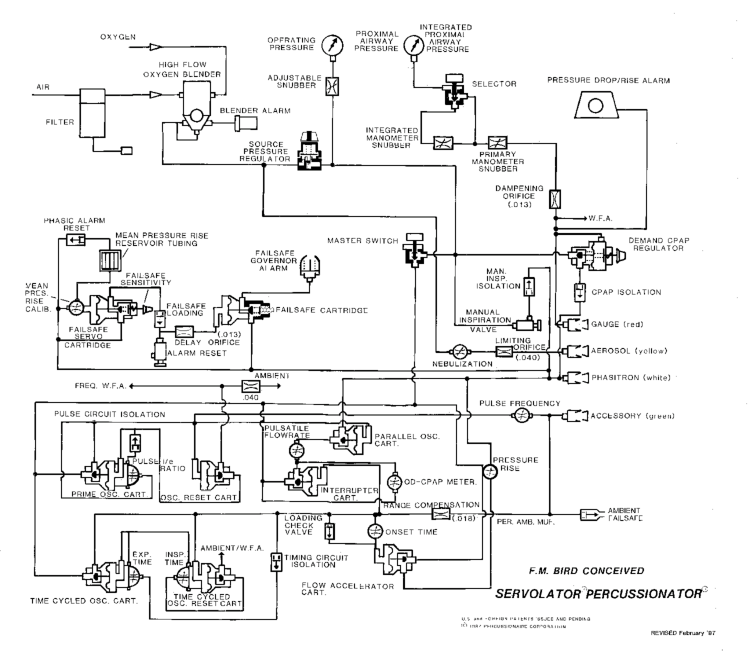
\includegraphics[height=\textheight]{img/circuit-logique.pdf}
	\note {Pas si logique que ça}
\end{frame}

\section{Analyse des tracés pression - temps}

\begin{frame}{Ratio I:E normal et inversé}
	\def\iehuit{%
\addplot graphics [
	xmin=0,
	ymin=0,
	xmax=1,
	ymax=60
]}

\begin{tikzpicture}

\begin{groupplot}[
group style={
	group size=1 by 2,
	xlabels at=edge bottom
},
enlargelimits=false,
height=0.46\textheight,
width=\textwidth,
xlabel=Temps (s),
ylabel=Pression (hPa)
]

\nextgroupplot
\iehuit {img/509.jpg};

\nextgroupplot
\iehuit{img/828.jpg};

\end{groupplot}
\end{tikzpicture}

\end{frame}

\begin{frame}{Ratio I:E normal et inversé}
	\def\iehuit{%
\addplot graphics [
	xmin=0,
	ymin=0,
	xmax=8,
	ymax=60
]}

\begin{tikzpicture}

\begin{groupplot}[
		group style={
			group size=1 by 2,
			xlabels at=edge bottom
		},
		enlargelimits=false,
		height=0.46\textheight,
		width=\textwidth,
		xlabel=Temps (s),
		ylabel=Pression (hPa)
]

\nextgroupplot
\iehuit {img/329.jpg};

\nextgroupplot
\iehuit {img/629.jpg};

\end{groupplot}
\end{tikzpicture}

\end{frame}

\begin{frame}{Augmentation des résistances}
	\centering
		\begin{tikzpicture}
		\begin{groupplot}[
				group style={
					group size=2 by 1
				},
				width=0.48\textwidth,
				restrict x to domain=1.5:4,
				every axis plot post/.style={
					mark=none
				},
				xlabel=Temps (s),
				ylabel=Pression (hPa),
				enlargelimits=false,
				ymax=40
			]
			\nextgroupplot[title=Résistances normales]
			\addplot table[x=time, y=Pao] {dat/raw5.dat};

		 \nextgroupplot[title=Résistances augmentées]
			\addplot table[x=time, y=Pao] {dat/raw15.dat};
		\end{groupplot}
	\end{tikzpicture}

\end{frame}

\end{document}
